\newpage
\section{Qualitative Design Discussion}
\label{app:solver}

Wall-clock time decomposition and search acceleration results are presented in Figure~\ref{fig:wallclock} and Section~\ref{sec:experiments}.


\subsection{Interesting Empirical Design Results}

\begin{table}[ht!]
\centering
\caption{Surprise design pairs discovered by CHEETAH-V1. Each pair achieves near-identical Perf/TDP via qualitatively different strategies that are not intuitive to human engineers.}
\label{tab:surprise_designs}
\resizebox{\textwidth}{!}{%
\begin{tabular}{llrrrrrrrrr}
\toprule
\textbf{Label} & \textbf{Workload} & \textbf{Trial} &
\textbf{Perf/TDP $\times$} & \textbf{Speedup $\times$} &
\textbf{MACs} & \textbf{CGM} &
\textbf{L1 in/w/o (KB)} & \textbf{L1 cfg} &
\textbf{L2 cfg} & \textbf{Batch} \\
\midrule
TPU-v3 ref   & --              & --  & 1.000 & 1.000  & 65{,}536  & 32 MB & 64 / 64 / 64     & Shared  & Disabled & 64  \\
\midrule
DeepSeek A   & \texttt{deepseek\_v3} & 81 & 3.158 & 25.125 & 524{,}288 & 8 MB  & 512 / 1 / 256    & Shared  & Disabled & 64  \\
DeepSeek B   & \texttt{deepseek\_v3} & 95 & 3.146 & 12.512 & 262{,}144 & 8 MB  & 1 / 256 / 512    & Shared  & Disabled & 128 \\
\midrule
Llama-3 70B A & \texttt{llama3\_70b} & 88 & 3.557 & 14.152 & 262{,}144 & 32 MB & 8 / 256 / 4      & Private & Shared   & 64  \\
Llama-3 70B B & \texttt{llama3\_70b} & 92 & 3.570 & 28.402 & 524{,}288 &  1 MB & 512 / 128 / 512  & Shared  & Shared   & 64  \\
\bottomrule
\end{tabular}%
}
\end{table}

We examine two designs on the DeepSeek-V3  (trials 81 vs.\ 95) and Llama-3 70B (trials 88 vs.\ 92) workloads. In each case, Perf/TDP scores are nearly identical yet design specifications are hugely different. DeekSeek's Design B uses 262K MACs vs.\ 524K in Design A. B compensates via richer search and larger batch. Pareto-tile space is 50$\times$ larger in B (500 vs.\ 10 configs); batch size doubles (128 vs.\ 64). Mirror-image L1 sub-buffer allocation in A keeps 512 KB input + 1 KB weight + 256 KB output. Design B keeps 1 KB input + 256 KB weight + 512 KB output. These two entirely opposite on-chip memory strategies yield identical system efficiency. On Llama-3 70B pair (trials 88 vs.\ 92), design A uses 262K MACs and 32 MB Global Buffer; Design B uses 524K MACs and only 1 MB Global Buffer. However Design A is weight-stationary, with a large 256 KB weight L1, tiny 8/4 KB input/output L1, and weight reuse amortised over a large on-chip scratchpad. Whereas Design B is activation-stationary, with 512/512 KB input/output L1, only 128 KB weight L1, and shared L1 configuration seen in doubled MACs allow CGM to collapse to 1 MB. This provides insight that additional compute in B substitutes for global memory capacity: higher throughput reduces the time activations must remain resident, relaxing the CGM capacity constraint. 


\subsection{Hardware and Vizier Search}

In all experiments, we utilize 16 NVIDIA H100 GPUs. Each unit in the configuration provides 80 GB of VRAM, totaling 1.28 TB of available memory across the cluster. The system is characterized by a high memory bandwidth of approximately 3.35 TB/s per GPU, which is critical for the memory-intensive workloads examined in this work. In order to be consistent with prior work on accelerator design \citep{zhang_fast}, we utilize Vizier to simulate TPUv3 and perform hardware search. \cref{tab:vizier_search_space} presents Vizier's search parameter groups for completeness, and \cref{fig:pipeline} depicts standard accelerator datapath configuration layout. 

A Processing Element (PE) is a repeated compute tile in an accelerator template.
The datapath can be modeled as a grid of PEs connected by a mesh on-chip network.
PE systolic arrays perform a matrix-vector multiply each cycle. 
Vector and scalar MACs are modeled by setting systolic array X and Y dimensions to 1. 
PEs also contain a VPU for non-MAC vector ops. 
L2 and Global Memory structures are optional. 

\begin{figure}[ht!]
    \centering
    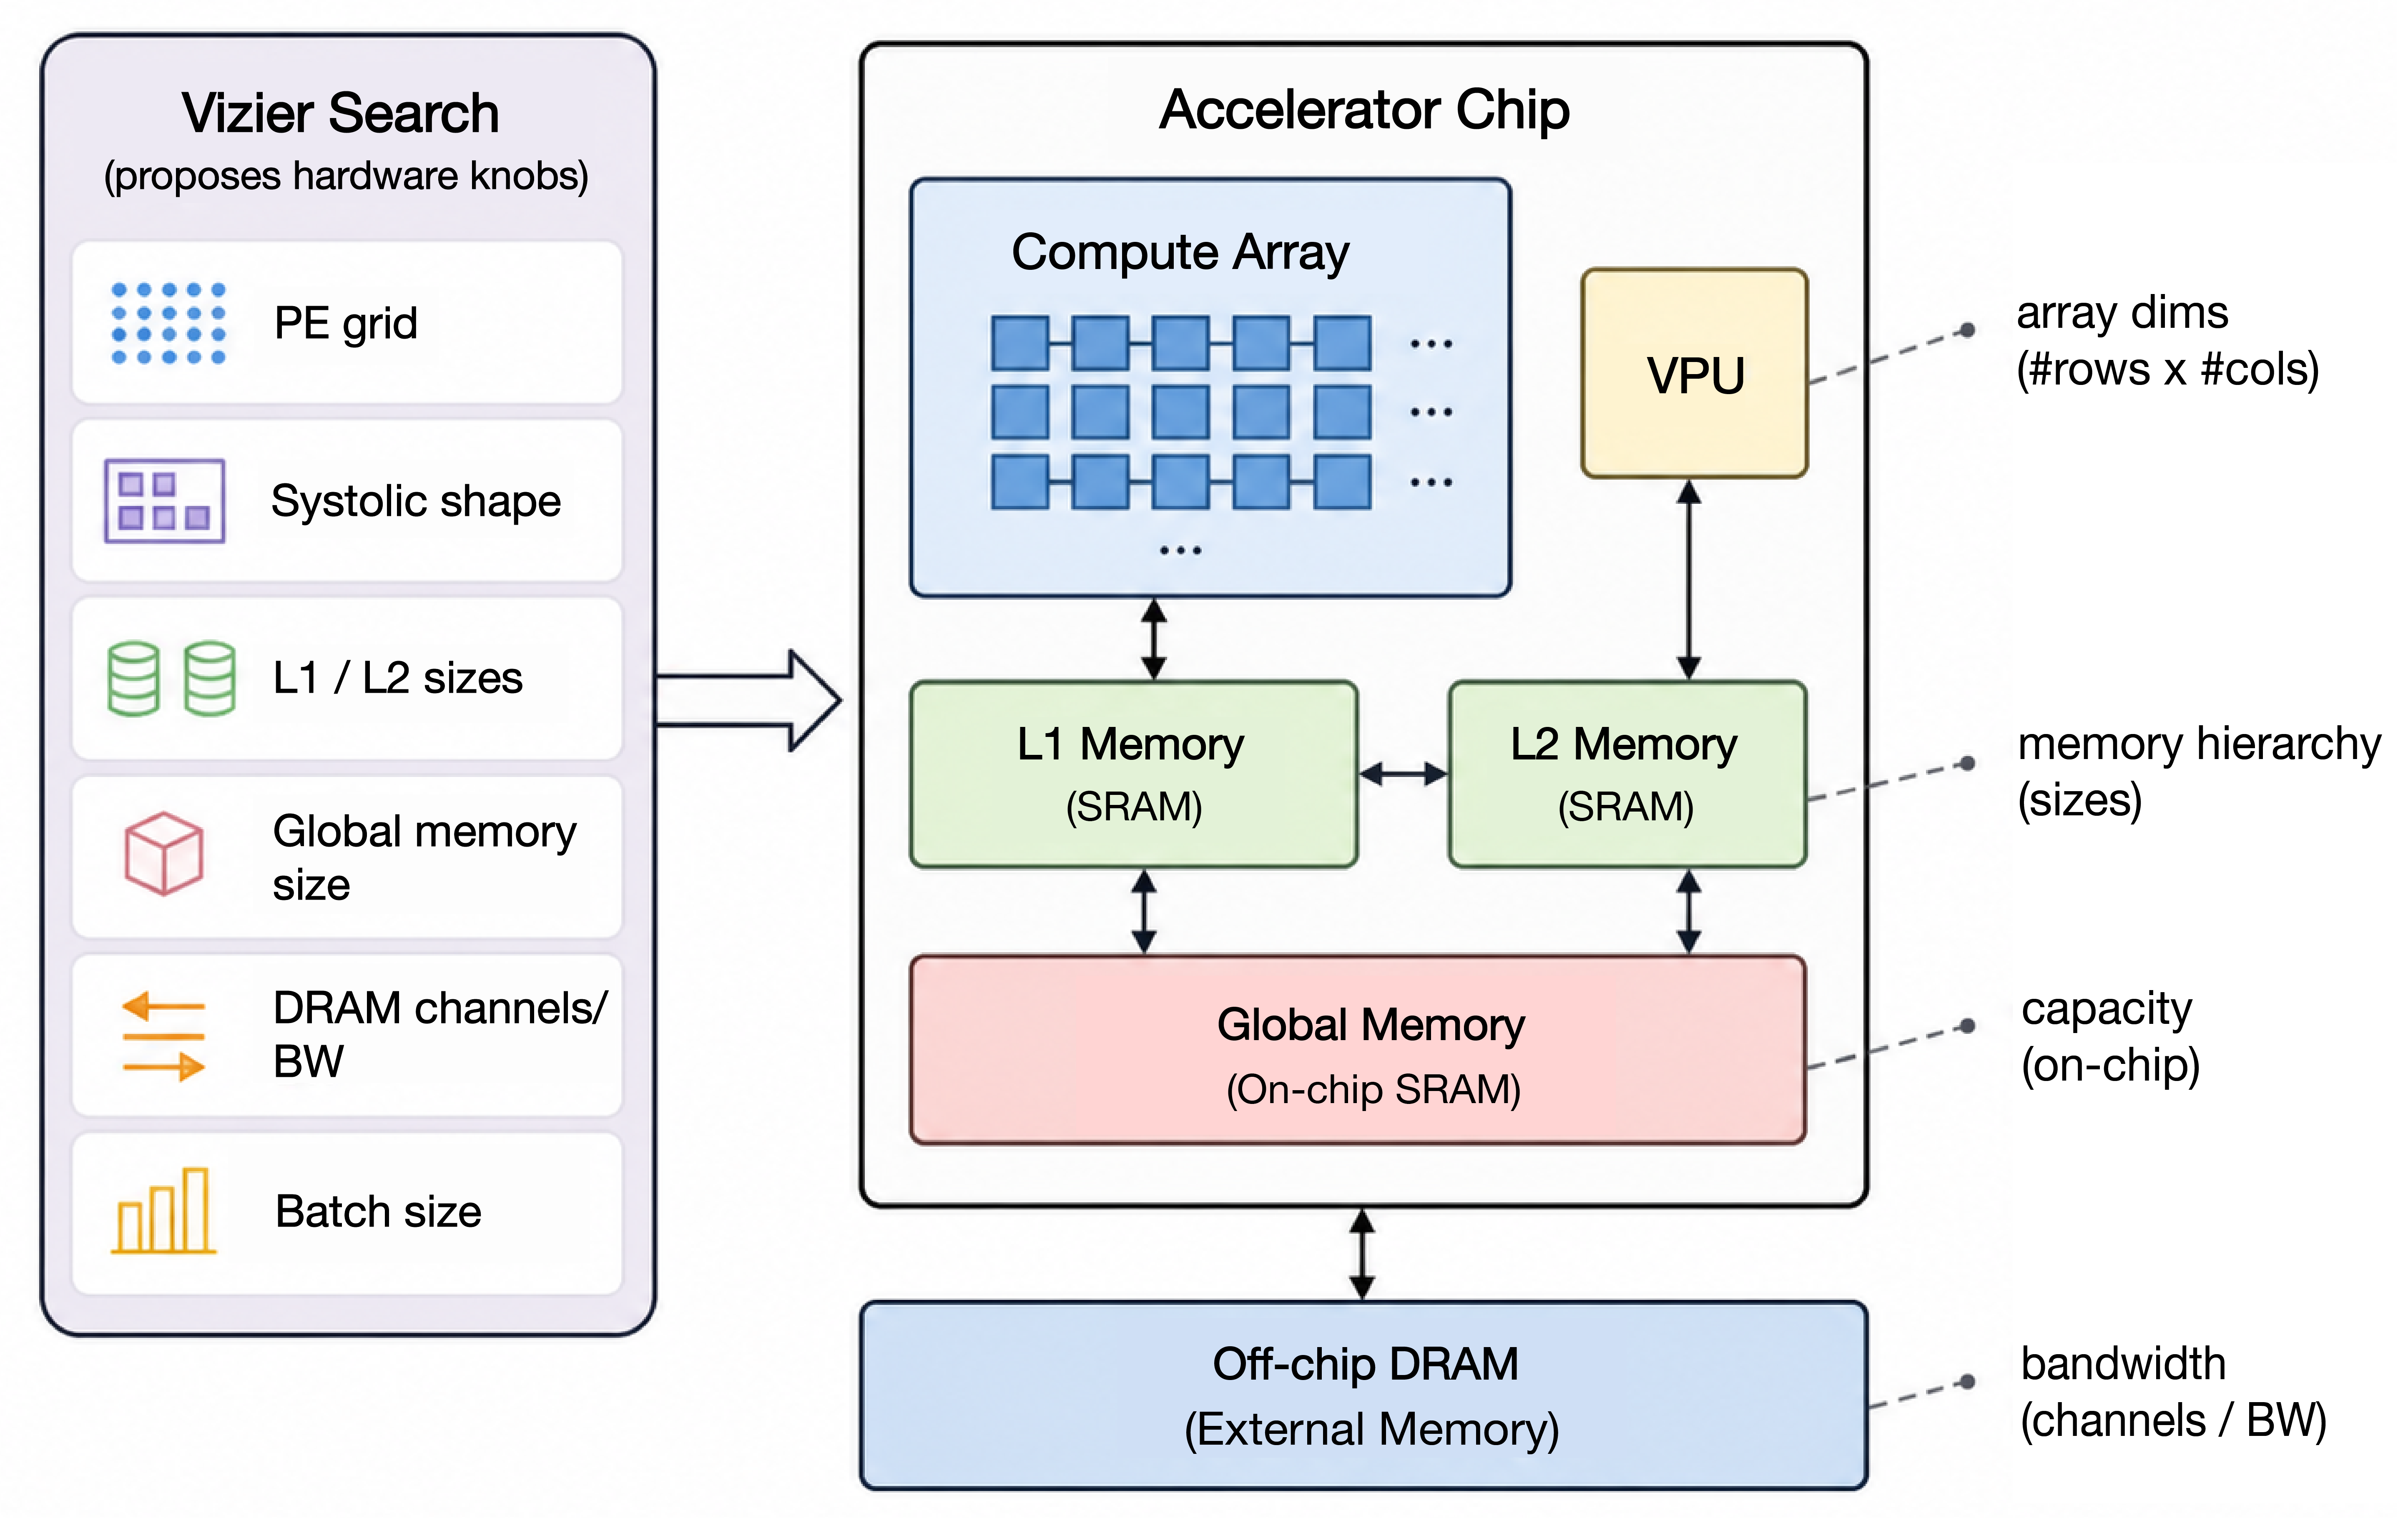
\includegraphics[width=0.7\linewidth]{figs/hardware_layout_v4.png}
    \caption{The accelerator datapath configuration. Processing elements (PEs) are arranged in a grid connected by a mesh network. Each PE contains a systolic array for matrix operations, a vector processing unit (VPU) for non-MAC operations, and private or shared L1/L2 memory. A Global Memory serves as the on-chip scratchpad shared across all PEs.}
    \label{fig:pipeline}
\end{figure}
\label{app:vizier}


\begin{table}[h]
\centering
\caption{Vizier search parameter groups and ranges: initial small search vs.\ expanded V1-wide search.}
\label{tab:vizier_search_space}
\resizebox{\textwidth}{!}{%
\begin{tabular}{llll}
\toprule
\textbf{Group} & \textbf{Parameter} & \textbf{Small (initial)} & \textbf{LLM-V1-wide} \\
\midrule
\multirow{16}{*}{\textbf{A: Hardware datapath (16 params)}}
 & \texttt{PEs\_x\_dim}                & pow2 in $\mathbf{4 \ldots 32}$                          & pow2 in $\mathbf{1 \ldots 256}$                        \\
 & \texttt{PEs\_y\_dim}                & pow2 in $\mathbf{4 \ldots 32}$                          & pow2 in $\mathbf{1 \ldots 256}$                        \\
 & \texttt{Systolic\_array\_x}         & pow2 in $\mathbf{4 \ldots 32}$                          & pow2 in $\mathbf{4 \ldots 128}$                        \\
 & \texttt{Systolic\_array\_y}         & pow2 in $\mathbf{4 \ldots 32}$                          & pow2 in $\mathbf{4 \ldots 128}$                        \\
 & \texttt{Vector\_unit\_multiplier}   & pow2 $1 \ldots 16$                                      & pow2 $1 \ldots 16$                                     \\
 & \texttt{L1\_buffer\_config}         & \{Private, Shared\}                                     & \{Private, Shared\}                                    \\
 & \texttt{L1\_input\_buffer\_size}    & pow2 $\mathbf{1\,\text{KB} \ldots 4\,\text{MB}}$        & pow2 $\mathbf{1\,\text{KB} \ldots 1\,\text{MB}}$       \\
 & \texttt{L1\_weight\_buffer\_size}   & pow2 $\mathbf{1\,\text{KB} \ldots 4\,\text{MB}}$        & pow2 $\mathbf{1\,\text{KB} \ldots 1\,\text{MB}}$       \\
 & \texttt{L1\_output\_buffer\_size}   & pow2 $\mathbf{1\,\text{KB} \ldots 4\,\text{MB}}$        & pow2 $\mathbf{1\,\text{KB} \ldots 1\,\text{MB}}$       \\
 & \texttt{L2\_buffer\_config}         & \{Disabled, Private, Shared\}                           & \{Disabled, Private, Shared\}                          \\
 & \texttt{L2\_input\_buffer\_mult.}   & pow2 $1 \ldots 128$                                     & pow2 $1 \ldots 128$                                    \\
 & \texttt{L2\_weight\_buffer\_mult.}  & pow2 $1 \ldots 128$                                     & pow2 $1 \ldots 128$                                    \\
 & \texttt{L2\_output\_buffer\_mult.}  & pow2 $1 \ldots 128$                                     & pow2 $1 \ldots 128$                                    \\
 & \texttt{L3\_global\_buffer} (CGM)   & $\{0\} \cup$ pow2 $\mathbf{1 \ldots 64\,\text{MB}}$     & $\{0\} \cup$ pow2 $\mathbf{1 \ldots 256\,\text{MB}}$   \\
 & \texttt{GDDR6\_channels}            & pow2 $\mathbf{1 \ldots 16}$ ($\to$ 64–1024 GB/s)        & pow2 $\mathbf{1 \ldots 32}$ ($\to$ 64–2048 GB/s)       \\
 & \texttt{Native\_batch\_size}        & pow2 $\mathbf{1 \ldots 1024}$                           & pow2 $\mathbf{1 \ldots 256}$                           \\
\midrule
\multirow{3}{*}{\textbf{B: Compiler passes (3 params)}}
 & \texttt{two\_pass\_softmax}         & \{disabled, enabled\}                                   & \{disabled, enabled\}                                  \\
 & \texttt{tensor\_padding}            & \{disabled, enabled\}                                   & \{disabled, enabled\}                                  \\
 & \texttt{datatype}                   & \{bfloat16, int8\}                                      & \{bfloat16, int8\}                                     \\
\midrule
\multirow{2}{*}{\textbf{C: V0 rematerialisation (2 params)}}
 & \texttt{remat\_enabled}             & \{disabled, enabled\}                                   & \{disabled, enabled\}                                  \\
 & \texttt{remat\_cost\_scale}         & \{0.1, 0.25, 0.5, 1.0, 2.0, 4.0\}                      & \{0.1, 0.25, 0.5, 1.0, 2.0, 4.0\}                     \\
\midrule
\multirow{4}{*}{\textbf{D: V1 joint-tiling (4 params)}}
 & \texttt{pareto\_config\_count\_C}   & \{10, 50, 100, 250, 500, 1000\}                         & \{10, 50, 100, 250, 500, 1000\}                        \\
 & \texttt{loop\_ordering\_strategy}   & \{weight\_stationary, output\_stationary, both\}        & \{weight\_stationary, output\_stationary, both\}       \\
 & \texttt{pareto\_pruning\_strategy}  & \{tmax\_workingset, tmax\_tmin, tmin\_workingset\}      & \{tmax\_workingset, tmax\_tmin, tmin\_workingset\}     \\
 & \texttt{tile\_workingset\_modeling} & \{fixed, config\_dep\}                                  & \{fixed, config\_dep\}                                 \\
\midrule
\multirow{4}{*}{\textbf{Post-Vizier gates (filter, not search)}}
 & \texttt{MIN\_TOTAL\_MACS}           & \multicolumn{2}{l}{$32{,}768$ ($4{\times}4{\times}4{\times}4{=}256$ lower physical, 32K gate)} \\
 & \texttt{MAX\_TOTAL\_MACS} cap       & none: implicit $\leq 32{\times}32{\times}32{\times}32 \approx 1\,\text{M}$ & $1{,}048{,}576$ explicit cap \\
 & Implied total\_MACs reach           & ${\approx}\,256 \ldots 1\,\text{M}$                     & $256 \ldots 1{,}048{,}576$ (post-cap)                  \\
 & Implied DRAM BW reach               & $64 \ldots 1{,}024$ GB/s                                & $64 \ldots 2{,}048$ GB/s                               \\
\bottomrule
\end{tabular}%
}
\end{table}